\documentclass[10pt,a4paper]{article}
\usepackage[utf8]{inputenc}
\usepackage{amsfonts}
\usepackage{amssymb}
\usepackage{float}
\usepackage{graphicx}
\usepackage{wrapfig}
\usepackage{hyperref}
\hypersetup{
    colorlinks,
    citecolor=black,
    filecolor=black,
    linkcolor=black,
    urlcolor=black,
    linktoc=all,
}
\date{}
\title{Paperwork manual}
% \setlength{\parskip}{\baselineskip}%

\begin{document}
\maketitle

WORK IN PROGRESS

\pagebreak

\tableofcontents

\pagebreak

\section{Settings}

\subsection{Accessing the settings}

\begin{figure}[H]
\begin{centering}
\includegraphics[scale=0.33]{out/app_menu.png}
\par\end{centering}
\caption{Application menu}
\end{figure}

Note that, on GNU/Linux, the application menu may be at the top of
the screen.

\begin{figure}[H]
\begin{centering}
\includegraphics[scale=0.5]{out/app_menu_opened.png}
\par\end{centering}
\caption{Settings}
\end{figure}


\subsection{Work directory}

\subsection{Scanner}

\subsubsection{Default scan source}

Some scanners have many sources/input. Basic scanners have only one
source : Flatbed. Some others have a feeder, allowing them to scan
many pages at one.

The settings here is the source to use for single scan.

If you select Flatbed here and use the
multi-scan dialog, Paperwork will
automatically switch to the feeder (if one is found ; otherwise the
default source is used too).

% \begin{figure}[H]
% \begin{centering}
% 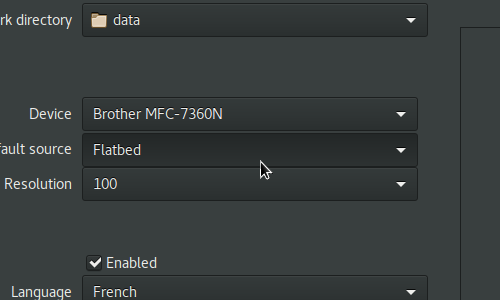
\includegraphics[scale=0.5]{img/generated/adf_settings}
% \par\end{centering}
% \caption{Selecting the default source for scanning}
% \end{figure}

% \begin{table}[H]
% \begin{centering}
% \begin{tabular}{|c|c|}
% \hline
% Flatbed only & 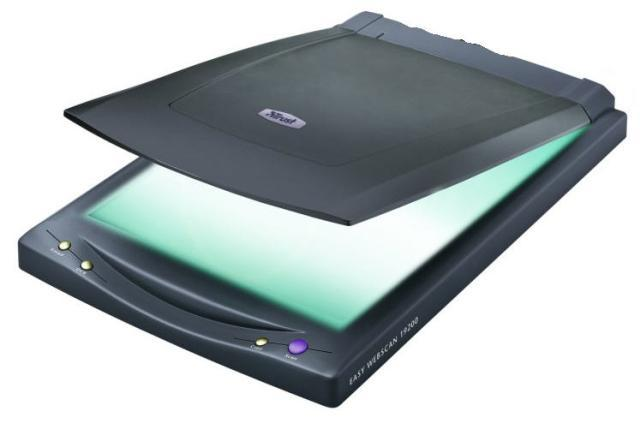
\includegraphics[scale=0.25]{img/flatbed}\tabularnewline
% \hline
% \hline
% Flatbed and feeder & 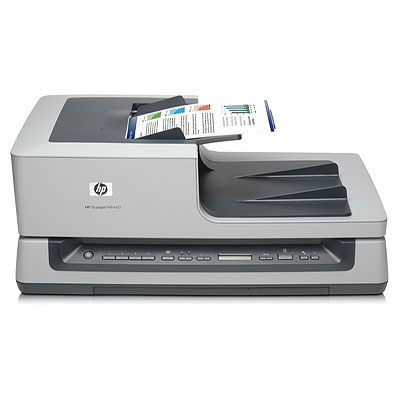
\includegraphics[scale=0.25]{img/flatbed_feeder}\tabularnewline
% \hline
% \end{tabular}
% \par\end{centering}
% \caption{Flatbeds and feeders}
% \end{table}

\subsubsection{Scanner calibration}

Scanners tend to provide images actually bigger than the scanned pages.
Since most of the time, you will always scan pages having the same
size (A4 or Letter usually), Paperwork provides an option called scanner
calibration. Scanner calibration in Paperwork is simply
a pre-cropping of the images coming from the scanner.

% \begin{figure}[H]
% \begin{centering}
% 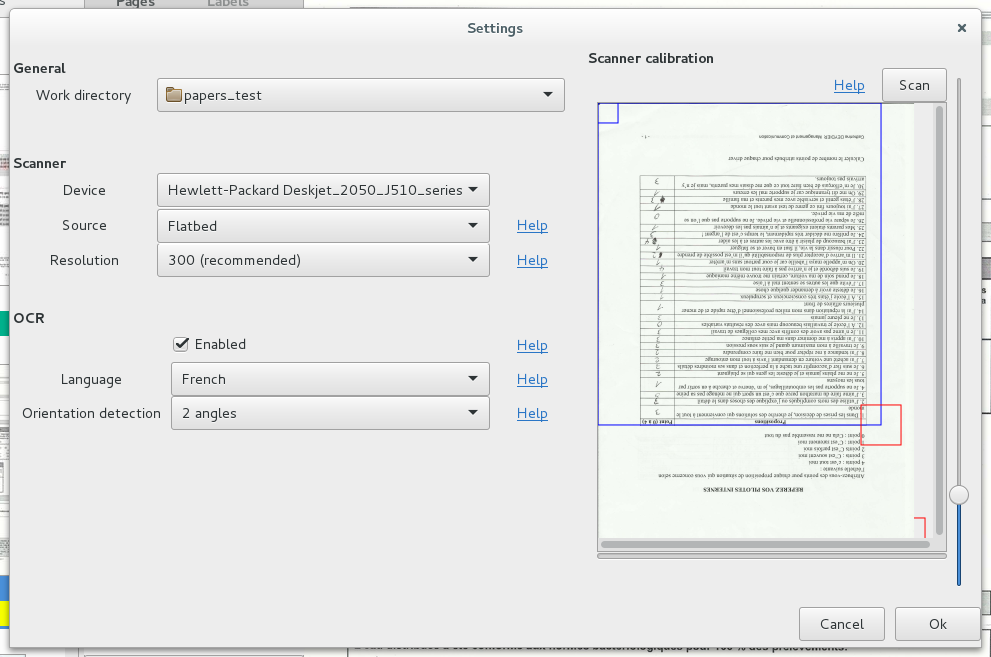
\includegraphics[width=1\columnwidth]{img/paperwork_settings_calibration}
%\par\end{centering}
% \caption{Scanner calibration}
% \end{figure}


\subsubsection{Scan resolution}

Scanner resolution defines how detailed the images coming from your
scanner must be.

Higher resolutions mean
\begin{itemize}
\item longer scans,
\item longer OCR,
\item more time to display,
\item more space used on disk,
\item but also better OCR.
\end{itemize}
Lower resolutions mean
\begin{itemize}
\item shorter scans,
\item shorter OCR,
\item less time to display,
\item less space used on disk,
\item but also inferior OCR,
\item and possibly unreadable image (even by a human).
\end{itemize}
300 dpi is considered a good trade-off. You may want to reduce it
to 200 dpi on slow computers.

\section{Scanning}

\subsection{Single scan}

% \begin{figure}[H]
% \begin{centering}
% 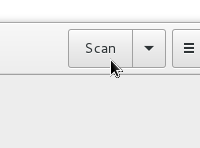
\includegraphics[scale=0.5]{img/generated/paperwork_scan}
% \par\end{centering}
% \caption{Scanning a single page}
% \end{figure}

Pages are appended to the current document.

\subsection{\label{subsec:From-feeder}From feeder}

% \begin{figure}[H]
% \begin{centering}
% 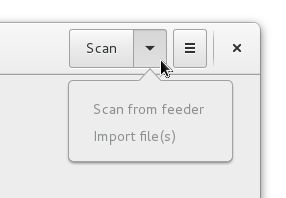
\includegraphics[scale=0.5]{img/generated/adf_access}
% \par\end{centering}
% \caption{Opening the dialog to scan from the feeder}
% \end{figure}

The option scan from feeder is enabled
only if Paperwork has detected a feeder on your scanner.

You have to tell Paperwork how many pages go in each document. If
you just want Paperwork to scan pages until none are left, you can
just specify a huge number of pages (99 for example).

% \begin{figure}[H]
% \begin{centering}
% 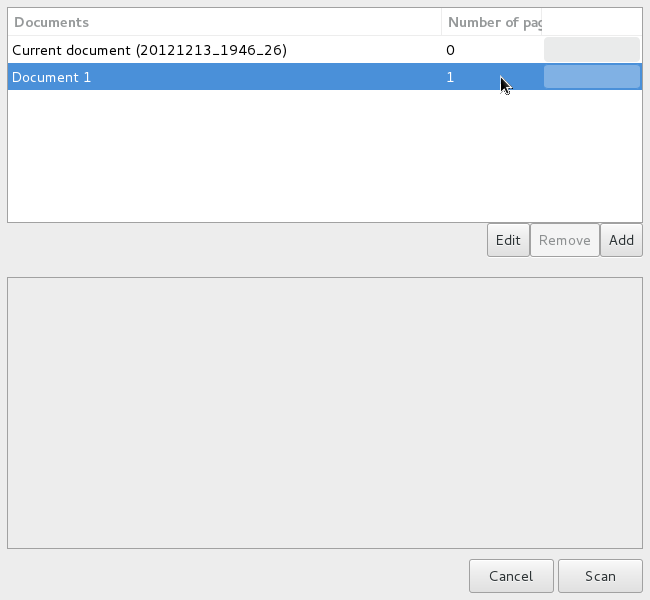
\includegraphics[width=1\columnwidth]{img/generated/adf_multiscan}
% \par\end{centering}
% \caption{Scanning multiple documents from the feeder}
% \end{figure}


\subsection{OCR languages}

By default, Paperwork uses Tesseract for the OCR. If unavailable,
it falls back on Cuneiform. On Windows, Tesseract is provided with
Paperwork.

To get better results, OCR tool need to know the language used in
the document(s).

The language available in the settings dialog of Paperwork are those
understood by the OCR tool. If your language is not in the list, it
means the OCR tool doesn't have the data required to read your language
and you must install them.

\subsubsection{Windows}

Tesseract and all its data files are provided by Paperwork's installer.
If a language is not available in the installer, it either means it
hasn't been packaged (in which case you can request it), or there
is no data file available yet for this language.

\subsubsection{Debian}
\begin{verbatim}
# OCR (Tesseract)
$ sudo apt-get install tesseract-ocr tesseract-ocr-<lang>
\end{verbatim}

\subsubsection{Fedora}
\begin{verbatim}
# OCR (Tesseract)
$ sudo dnf install tesseract tesseract-langpack-<lang>
\end{verbatim}

\subsubsection{Ubuntu}
\begin{verbatim}
# OCR (Tesseract)
$ sudo apt-get install tesseract-ocr tesseract-ocr-<lang> 
\end{verbatim}

\subsection{OCR enabled / disabled}

When you scan a page using Paperwork, Paperwork will immediately run
the OCR on it. This process may take a while for each page.

In case you want to scan a lot of pages quickly (for instance, the
first time you use Paperwork), OCR can be temporarily disabled.

% \begin{figure}[H]
% \begin{minipage}[t]{0.45\columnwidth}%
% \begin{flushright}
% 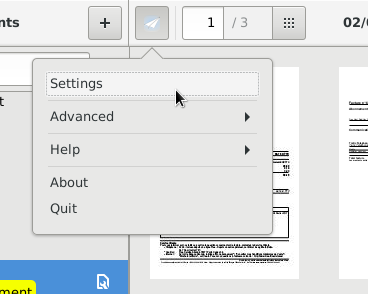
\includegraphics[scale=0.3]{img/menu_settings}
% \par\end{flushright}%
% \end{minipage} %
% \begin{minipage}[t]{0.45\columnwidth}%
% 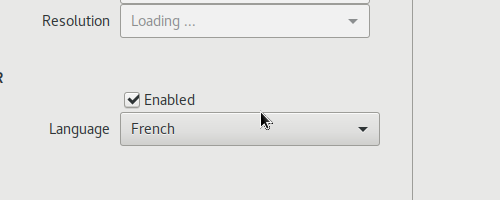
\includegraphics[scale=0.3]{img/generated/settings_disable_ocr}%
% \end{minipage}
% \caption{Disabling the OCR}
% \end{figure}

OCR can then be run on all the documents managed by Paperwork in one
shot.

% \begin{figure}[H]
% \begin{minipage}[t]{0.45\columnwidth}%
% \begin{flushright}
% 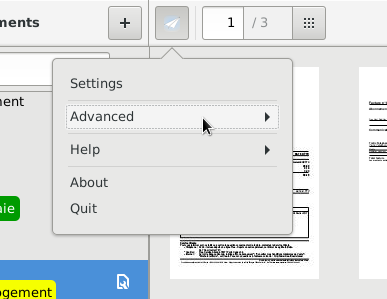
\includegraphics[scale=0.33]{img/menu_advanced}
% \par\end{flushright}%
% \end{minipage} %
% \begin{minipage}[t]{0.45\columnwidth}%
% 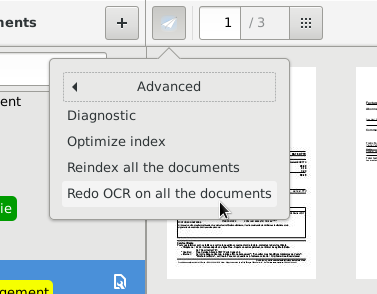
\includegraphics[scale=0.33]{img/menu_advanced_redo_ocr_all}%
% \end{minipage}
% \caption{Redo OCR on all the documents}
% \end{figure}


\section{Importing}

% \begin{figure}[H]
% \begin{minipage}[t]{0.45\columnwidth}%
% \begin{flushright}
% 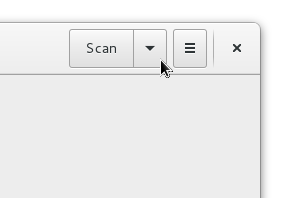
\includegraphics[scale=0.5]{img/generated/import_pdf_en_0001}
% \par\end{flushright}%
% \end{minipage} %
% \begin{minipage}[t]{0.45\columnwidth}%
% 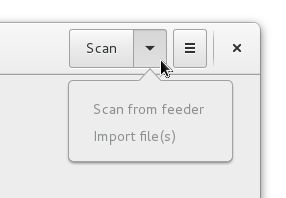
\includegraphics[scale=0.5]{img/generated/import_pdf_en_0002}%
% \end{minipage}\caption{Import option}
% \end{figure}

% \begin{figure}[H]
% \begin{centering}
% 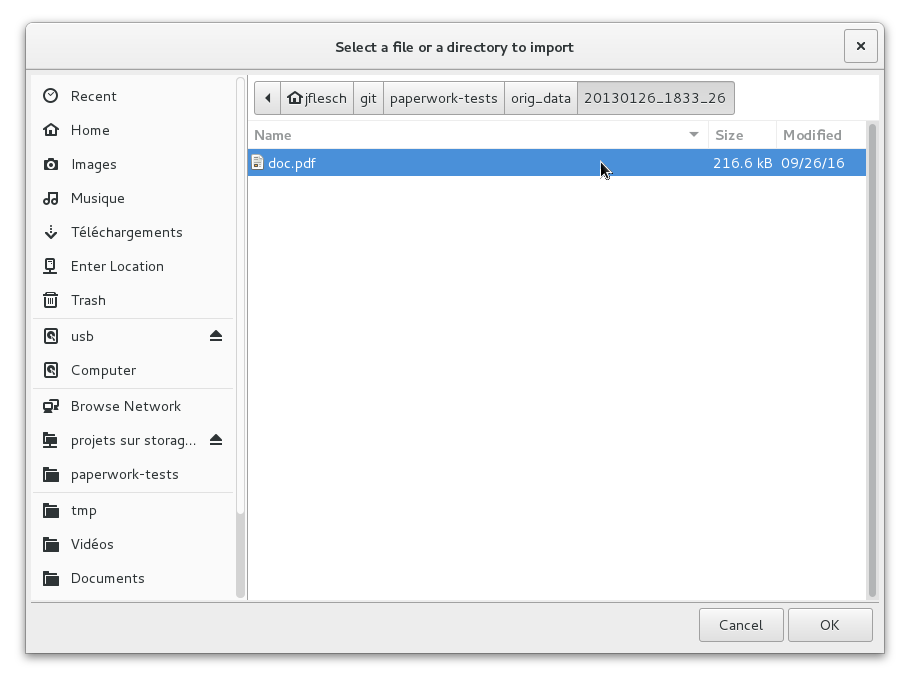
\includegraphics[width=1\columnwidth]{img/generated/import_pdf_en_0003}
% \par\end{centering}
% \caption{Select a file or a folder}
% \end{figure}


\subsection{Images}

Paperwork supports a lot of file formats. It supports JPEG, PNG, GIF,
BMP, TIFF, etc.

Each image is considered as a page. Currently, you can only import
one file at a time.

Images are always appended to the document currently opened. Simply
select an empty document ("New document") to create a new document while
importing.

OCR is always run on imported images. If the imported image is the
first page of a new document, Paperwork will automatically apply documents
labels.

Note that Paperwork is a document manager. While it can, it is not
designed to handle images with only very little text or photos. Automatic
labeling will not work correctly on such documents.

The OCR (Tesseract) works very well with black text on white background.
Automatic labeling uses recognized text and requires as many keywords
on the first page as possible.

\subsection{PDF}

Each PDF is always considered as a whole document. They are never
appended to existing document. They are copied as is in the work directory
and are never modified by Paperwork (just moved and renamed).

Paperwork will look for pages with no text attached. On those pages,
it will automatically run OCR. Once all the pages have been examined,
it will automatically apply document labels. Note that this process
may take a few minutes for big PDFs files.

If the PDF is already part of your documents, Paperwork will simply
ignore it.

\subsection{Many PDFs in one shot}

If you import a folder, Paperwork will browse this folder and look
for PDFs to import. Already-imported PDFs are simply ignored. Folder
is browsed recursively (all the folders inside the folder are also
examined).

\section{Labels}

\subsection{Creating new labels}

% \begin{figure}[H]
% \begin{doublespace}
% \begin{minipage}[t]{0.45\columnwidth}%
% \begin{flushright}
% 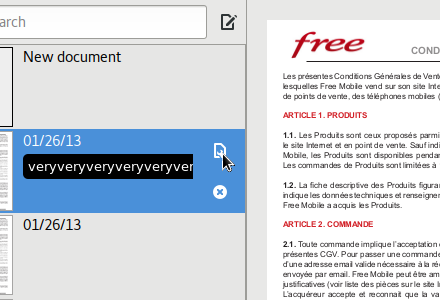
\includegraphics[scale=0.3]{img/generated/paperwork_goto_labels_and_memo}
% \par\end{flushright}%
% \end{minipage} %
% \begin{minipage}[t]{0.45\columnwidth}%
% 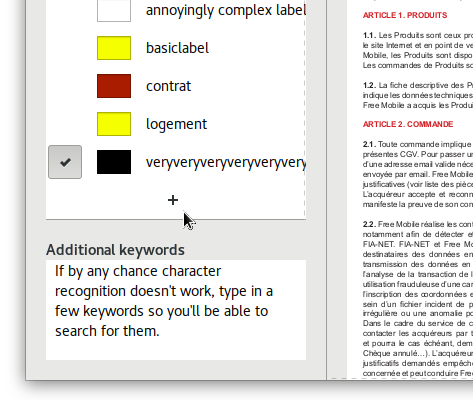
\includegraphics[scale=0.3]{img/generated/add_label}%
% \end{minipage}
% \end{doublespace}
% \begin{centering}
% 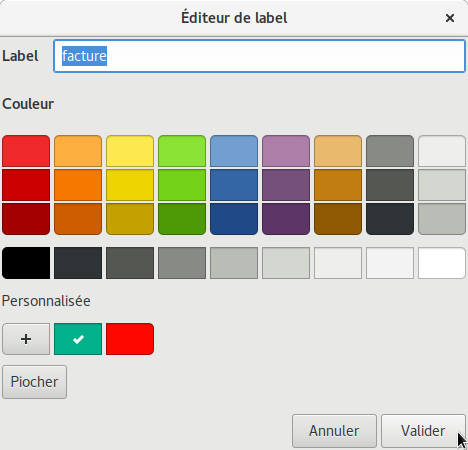
\includegraphics[scale=0.33]{img/label_editor}
% \par\end{centering}
% \caption{Creating a new label}
% \end{figure}


\subsection{Setting labels on documents}

% \begin{figure}[H]
% \begin{doublespace}
% \begin{minipage}[t]{0.45\columnwidth}%
% \begin{flushright}
% 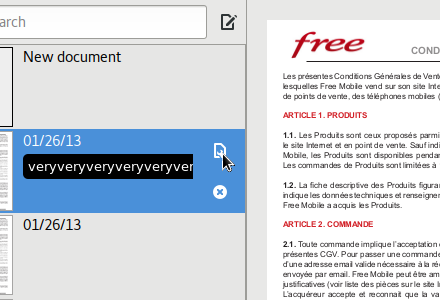
\includegraphics[scale=0.3]{img/generated/paperwork_goto_labels_and_memo}
% \par\end{flushright}%
% \end{minipage} %
% \begin{minipage}[t]{0.45\columnwidth}%
% 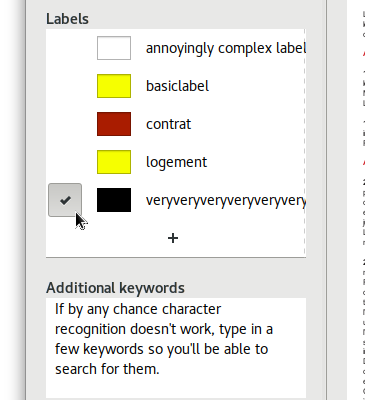
\includegraphics[scale=0.3]{img/generated/label_select}%
% \end{minipage}
% \end{doublespace}
% \caption{Selecting a label}
% \end{figure}


\subsection{Modifying a label}

% \begin{figure}[H]
% \begin{doublespace}
% \begin{minipage}[t]{0.45\columnwidth}%
% \begin{flushright}
% 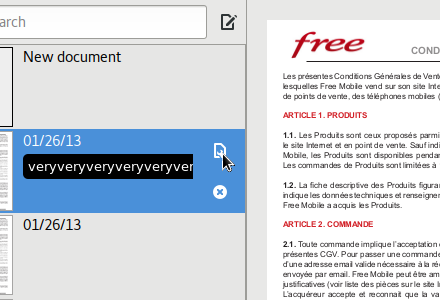
\includegraphics[scale=0.3]{img/generated/paperwork_goto_labels_and_memo}
% \par\end{flushright}%
% \end{minipage} %
% \begin{minipage}[t]{0.45\columnwidth}%
% 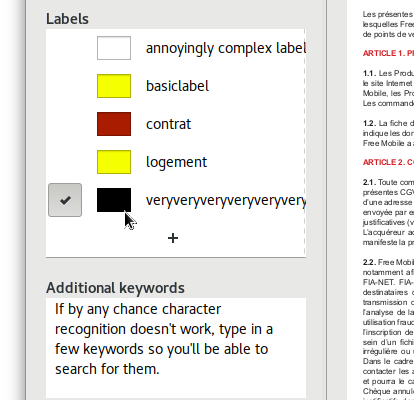
\includegraphics[scale=0.3]{img/generated/label_goto_edit}%
% \end{minipage}
% \end{doublespace}
% \begin{centering}
% 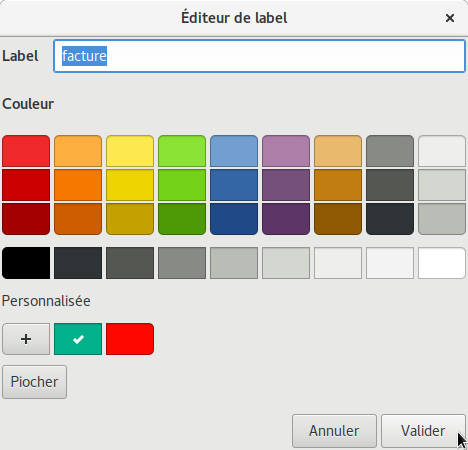
\includegraphics[scale=0.3]{img/label_editor}
% \par\end{centering}
% \caption{Modifying a label}
% \end{figure}


\subsection{Deleting a label}

%\begin{figure}[H]
%\begin{doublespace}
%\begin{minipage}[t]{0.45\columnwidth}%
%\begin{flushright}
%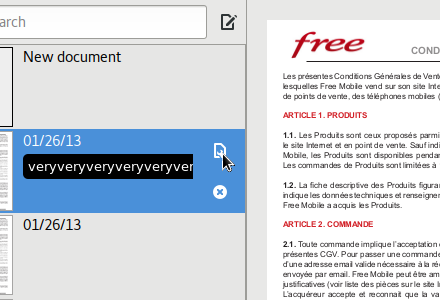
\includegraphics[scale=0.3]{img/generated/paperwork_goto_labels_and_memo}
%\par\end{flushright}%
%\end{minipage} %
%\begin{minipage}[t]{0.45\columnwidth}%
%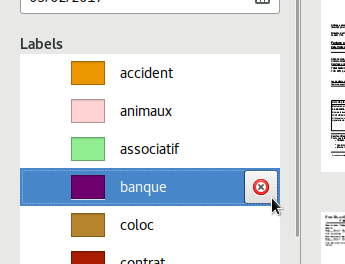
\includegraphics[scale=0.3]{img/label_delete}%
%\end{minipage}
%\end{doublespace}
%\caption{Deleting a label}
%\end{figure}


\section{Searching}

\subsection{Simple search}

%\begin{figure}[H]
%\begin{centering}
%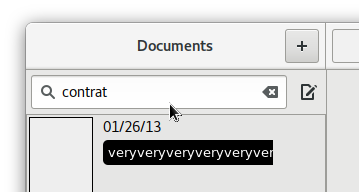
\includegraphics[scale=0.5]{img/generated/paperwork_search}
%\par\end{centering}
%\caption{Searching}
%\end{figure}


\subsection{Advanced search}

%\begin{figure}[H]
%\begin{centering}
%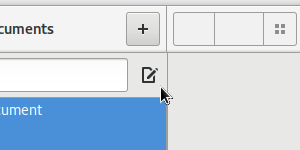
\includegraphics[scale=0.3]{img/generated/goto_advanced_search} 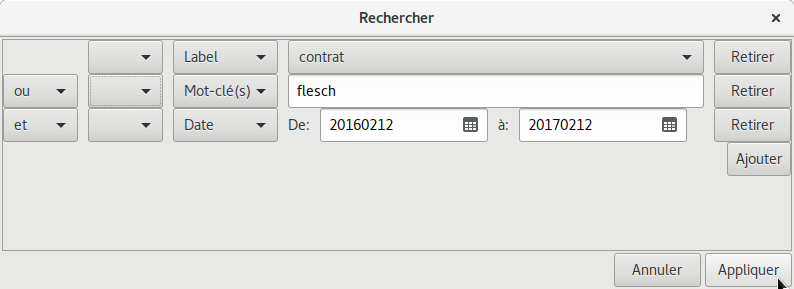
\includegraphics[scale=0.3]{img/search_advanced}
%\par\end{centering}
%\caption{Advanced search}
%\end{figure}


\section{Viewing}

\subsection{View pages as grid}

%\begin{figure}[H]
%\begin{centering}
%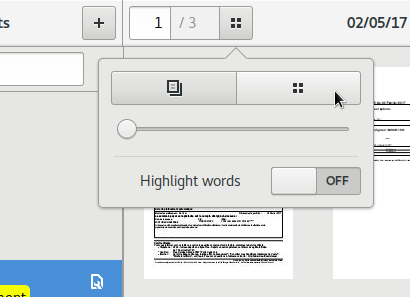
\includegraphics[scale=0.3]{img/view_grid}
%\par\end{centering}
%\caption{Switch to grid layout}
%\end{figure}


\subsection{View pages as list}

%\begin{figure}[H]
%\begin{centering}
%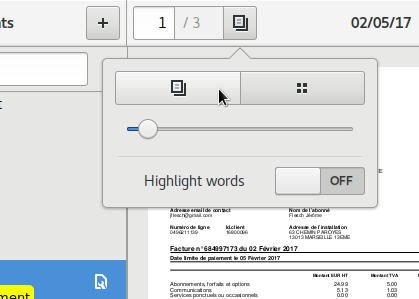
\includegraphics[scale=0.3]{img/view_paged}
%\par\end{centering}
%\caption{Switch to list layout}
%\end{figure}


\subsection{Zoom level}

%\begin{figure}[H]
%\begin{centering}
%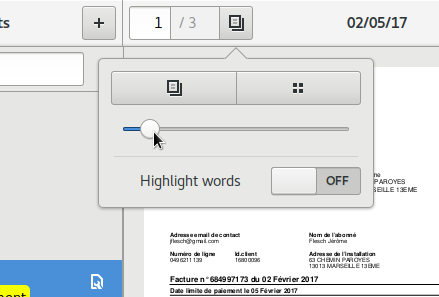
\includegraphics[scale=0.3]{img/view_zoom}
%\par\end{centering}
%\caption{Changing zoom level}
%\end{figure}


\section{Exporting}

%\begin{figure}[H]
%\begin{centering}
%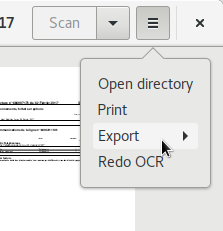
\includegraphics[scale=0.3]{img/paperwork_export_0001} 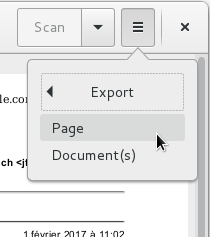
\includegraphics[scale=0.3]{img/paperwork_export_0002}
%\par\end{centering}
%\caption{Exporting}
%\end{figure}


\subsection{Document}

\subsection{Page}

\section{Printing}

%\begin{figure}[H]
%\begin{centering}
%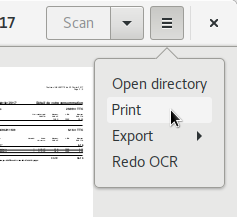
\includegraphics[scale=0.4]{img/menu_print}
%\par\end{centering}
%\caption{Printing}
%\end{figure}

\section{Copying text}

\section{Editing pages}

%\begin{figure}[H]
%\begin{centering}
%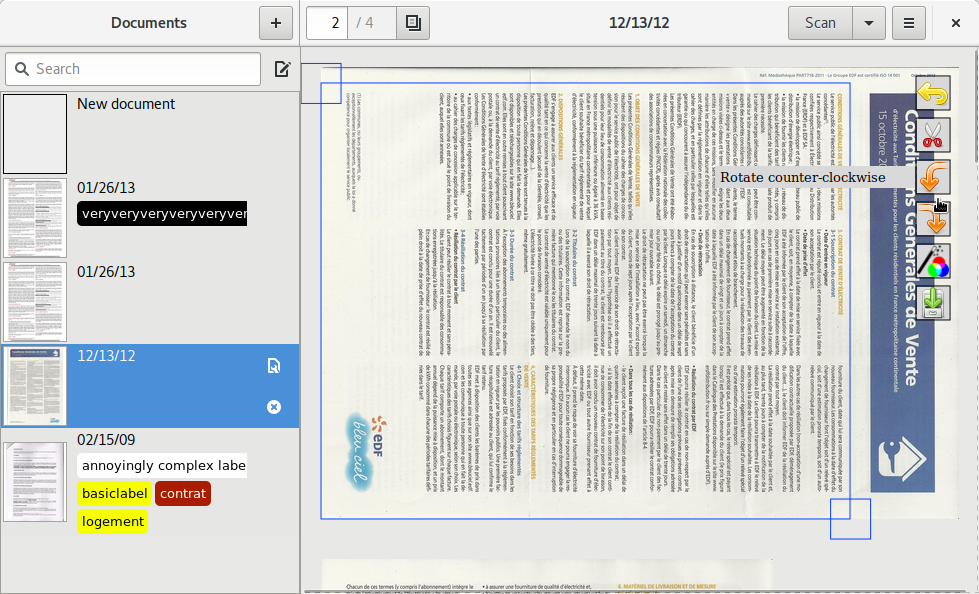
\includegraphics[width=1\columnwidth]{img/page_edit}
%\par\end{centering}
%\caption{Page editing}
%\end{figure}

\section{Moving pages}

\subsection{inside a document}

\subsection{from a document to another}

\section{Switching to another work directory}

Before copying or moving the work directory of Paperwork, please close
Paperwork.

When Paperwork starts, on of the first things it does is to look for
any change in its current work directory. Therefore, if you moved
your work directory, when you will restart Paperwork, since it won't
find anything, the document list will be empty.

You must then go in the settings and change the work directory location
to the new one.

In the following example, we are switching to a work directory contained
in a DropBox's folder :

%\begin{figure}[H]
%\begin{centering}
%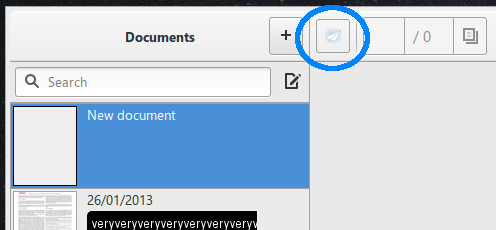
\includegraphics[scale=0.5]{img/change_workdir_en_0002}
%\par\end{centering}
%\caption{Application menu}
%\end{figure}
%
Note that, on GNU/Linux, the application menu may be at the top of
the screen.

%\begin{figure}[H]
%\begin{centering}
%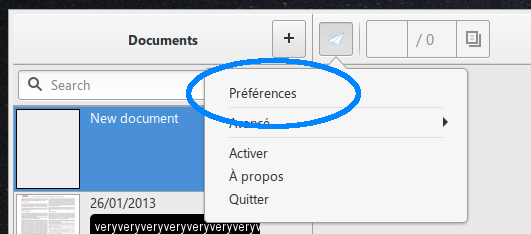
\includegraphics[scale=0.5]{img/change_workdir_en_0003}
%\par\end{centering}
%\caption{Settings}
%\end{figure}

%\begin{figure}[H]
%\begin{doublespace}
%\begin{minipage}[t]{0.45\columnwidth}%
%\begin{flushright}
%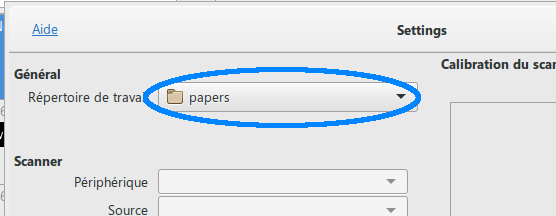
\includegraphics[scale=0.4]{img/change_workdir_en_0004}
%\par\end{flushright}%
%\end{minipage} %
%\begin{minipage}[t]{0.45\columnwidth}%
%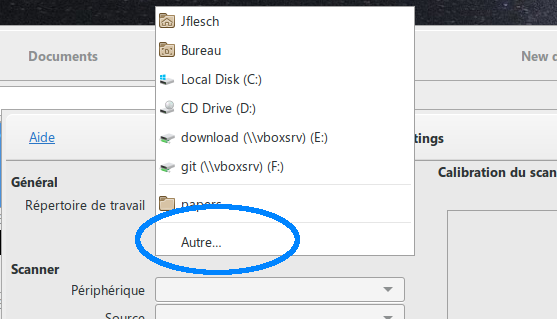
\includegraphics[scale=0.4]{img/change_workdir_en_0005}%
%\end{minipage}

%\begin{minipage}[t]{1\columnwidth}%
%\begin{center}
%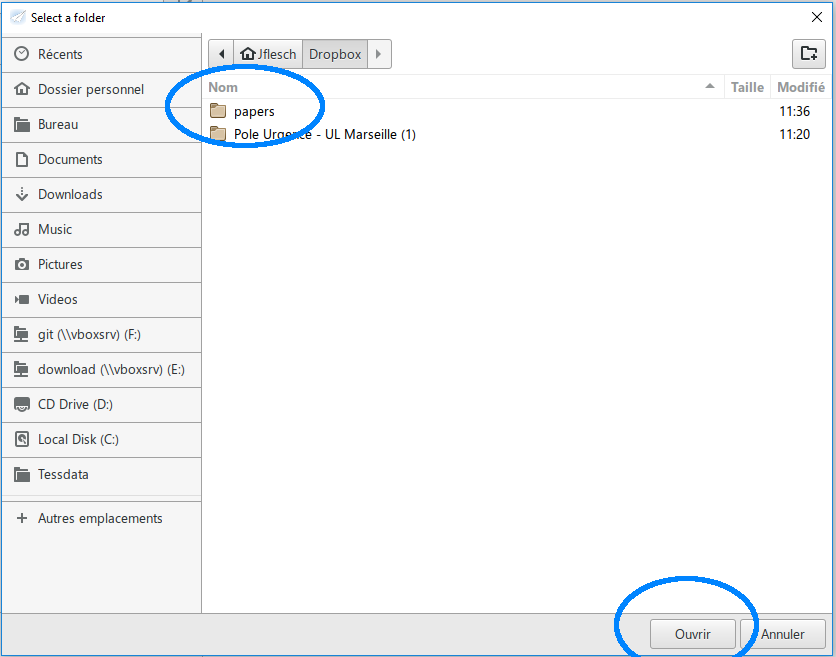
\includegraphics[scale=0.4]{img/change_workdir_en_0008}
%\par\end{center}%
%\end{minipage}
%\end{doublespace}
%\begin{minipage}[t]{1\columnwidth}%
%\end{minipage}
%\caption{Work directory selection}
%\end{figure}

%\begin{figure}[H]
%\begin{centering}
%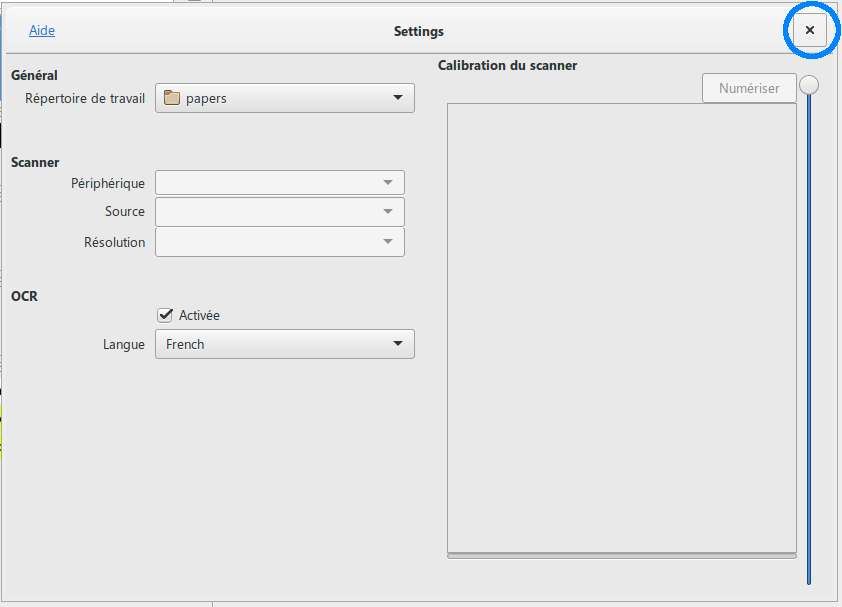
\includegraphics[scale=0.5]{img/change_workdir_en_0010}
%\par\end{centering}
%\caption{Apply new settings}
%\end{figure}

Paperwork will automatically scan the newly selected work directory,
and update its index according to its content.

\section{Backup}

\section{Synchronisation}

While Paperwork is a personal document manager, it is not a file synchronization
application. However, it is designed to be used with file synchronization
applications (Dropbox, OneDrive, Owncloud, SparkleShare, etc).

When you start Paperwork, one of the first things it does is check
the content of the work directory. It looks for any changes and updates
its document list and index accordingly, automatically.

\subsection{USB key / USB drive}

This is the simplest way to share documents. Simply copy your work
directory to an USB key, tell Paperwork to use it, and you're done.

Beware: You should backup your USB key from time to time on another
one.

\subsection{File Synchronization applications}

Those applications synchronize a local directory with a remote server
(or cloud). All the changes you do in your folder are applied on the
server. All the changes applied on the servers are applied to the
computers that connect to it. The server can belong to you or to someone
else (usually a company).

Beware: If you choose to host your documents on someone else server
(DropBox, OneDrive, etc), they can access all your documents. Paperwork
does not cipher them.

Paperwork is tested daily with SparkleShare. While this is not the
easiest one to use, Sparkleshare let you host your files yourself.
Using DropBox or OneDrive can make sense if you're sharing not-so-confidential
documents with others (associations, etc).

\subsubsection{DropBox}

Here we are detailing the process to use DropBox, but it is similar
for other file synchronization applications.

First, you must copy or move your work directory inside the DropBox
folder (please stop Paperwork before):

%\begin{figure}[H]
%\centering{}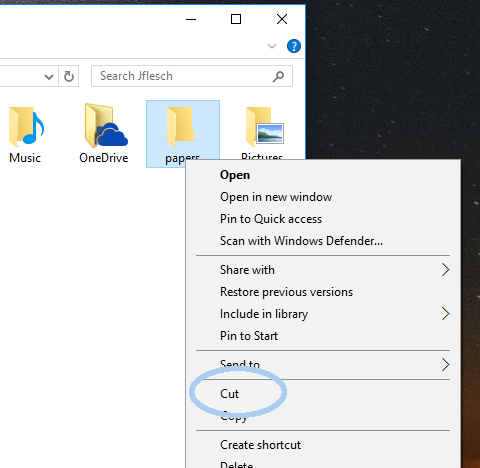
\includegraphics[scale=0.5]{img/sharing_dropbox_en_0001}
%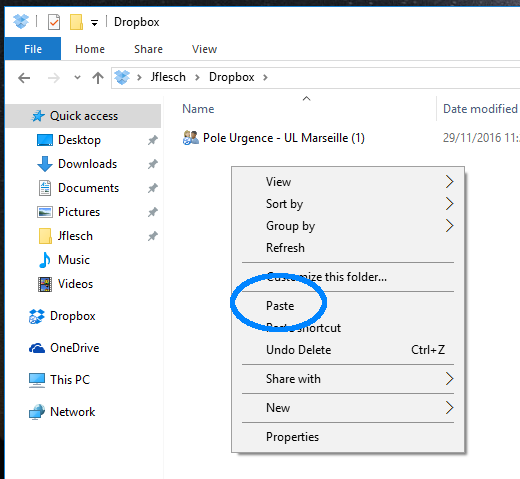
\includegraphics[scale=0.5]{img/sharing_dropbox_en_0002}\caption{Cut and paste paperwork work directory into the shared directory}
%\end{figure}

Then you must tell Paperwork to use this new work directory.

\subsubsection{Shared folder}

If all your computers are on the same network, you can share your
work directory. However, be really careful regarding permissions.
Being too permissive could let a pirate access all your personal documents
! And setting them correctly is tricky.

Beware: While file synchronization applications usually maintain an
historic, shared folders do not. You should do backups from time to
time.

\paragraph{Here are the instructions for Microsoft Windows:}

%\begin{figure}[H]
%\begin{centering}
%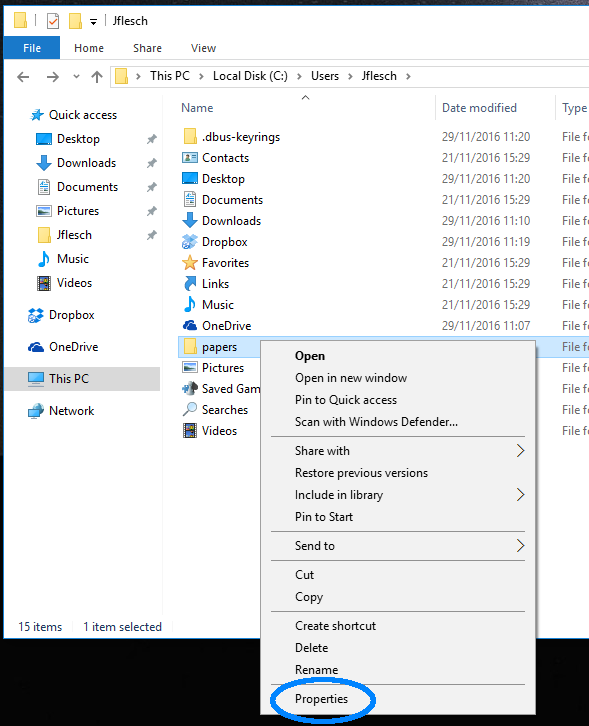
\includegraphics[scale=0.5]{img/sharing_network_folder_en_0001}
%\par\end{centering}
%\caption{Go to the properties of the work directory}
%\end{figure}
%
%\begin{figure}[H]
%\begin{centering}
%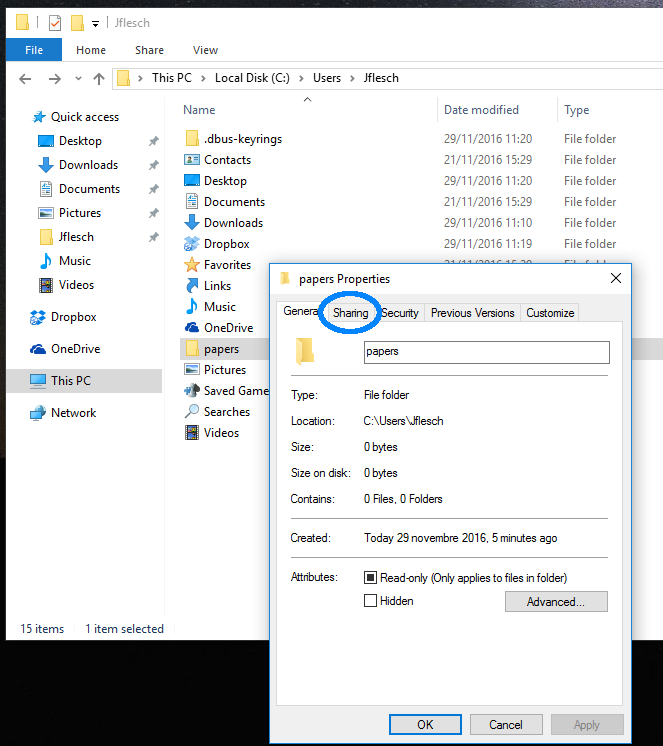
\includegraphics[scale=0.5]{img/sharing_network_folder_en_0002}
%\par\end{centering}
%\caption{Go to the tab ``Sharing''}
%\end{figure}
%
%\begin{figure}[H]
%\begin{centering}
%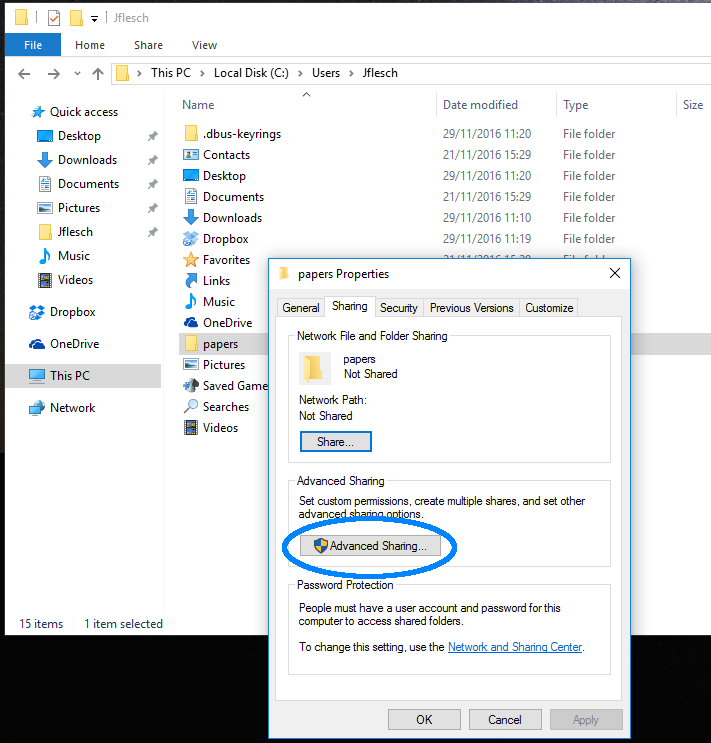
\includegraphics[scale=0.5]{img/sharing_network_folder_en_0003}
%\par\end{centering}
%\caption{Go to ``Advanced Sharing''}
%
%\end{figure}
%
%\begin{figure}[H]
%\begin{centering}
%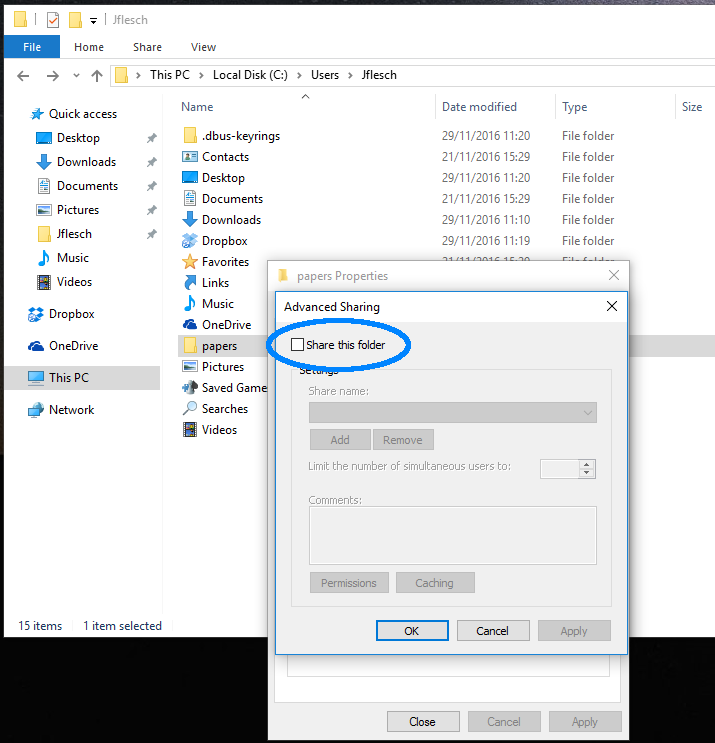
\includegraphics[scale=0.5]{img/sharing_network_folder_en_0004}
%\par\end{centering}
%\caption{Check ``Share this folder''}
%
%\end{figure}
%
%\begin{figure}[H]
%\centering{}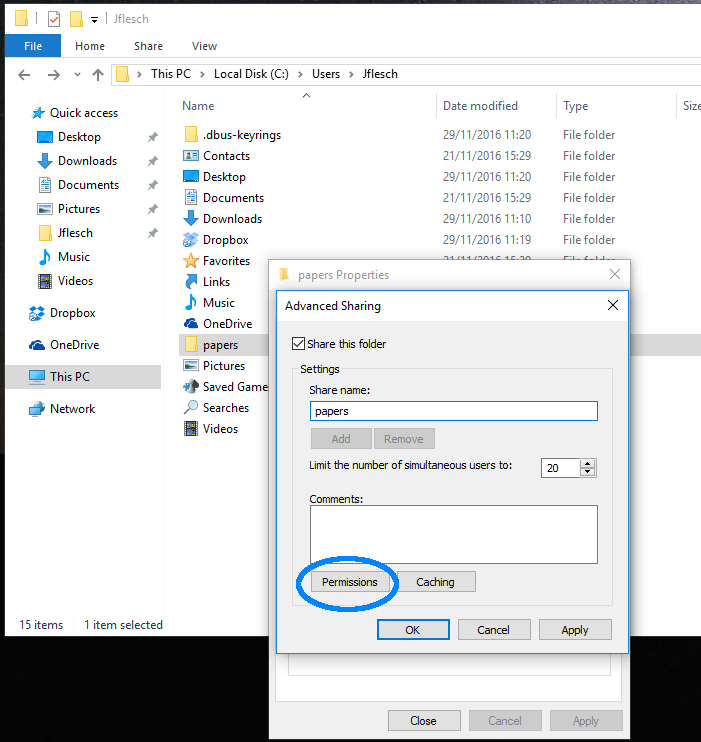
\includegraphics[scale=0.5]{img/sharing_network_folder_en_0005}\caption{Go to the permissions}
%\end{figure}
%
%\begin{figure}[H]
%\centering{}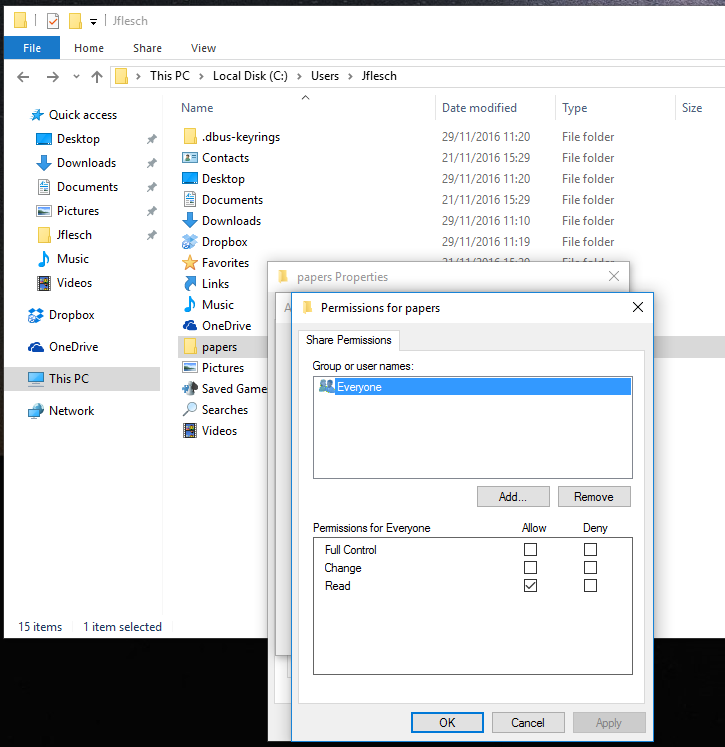
\includegraphics[scale=0.5]{img/sharing_network_folder_en_0006}\caption{Set the permissions as you wish}
%\end{figure}
%

\paragraph{On the client side, you must map the shared folder to a drive.}

%\begin{figure}[H]
%\centering{}\includegraphics[scale=0.5]{img/sharing_network_folder_en_0007}\caption{You must map a network drive}
%\end{figure}
%
%\begin{figure}[H]
%\begin{centering}
%\includegraphics[scale=0.5]{img/sharing_network_folder_en_0008}
%\par\end{centering}
%\caption{Network drive setup}
%
%\end{figure}
%

\section{Encryption}

\subsection{Windows}

TODO


\subsection{GNU/Linux}

GNU/Linux distributions include many tools to encrypt whole directories.

With Paperwork, there are 2 directories that should be encrypted to
protect your privacy:
\begin{itemize}
\item Your work directory (by default \textasciitilde /papers, can be changed
in the settings)
\item The cache directory (\textasciitilde /.local/share/paperwork, cannot
be changed) (it contains index files from which the content of your
documents could be partially recovered)
\end{itemize}

Note that if you want to be sure that your data are always encrypted,
it's recommended to encrypt your whole home directory or even your whole system
if possible.

\subsubsection{Ecryptfs}

On GNU/Linux Debian and Ubuntu, you can easily create a directory
Private in your home directory. This directory will be encrypted using
the password you use to connect when you start your computer. Just
type ecryptfs-setup-private in a terminal to create it. You have to
logout/login agan. You can then put the work directory of Paperwork
in it.

Once the directory has been created, you can also store Paperwork
index in it:
\begin{verbatim}
$ mv ~/.local/share/paperwork ~/Private/paperwork_index
$ ln -s ~/Private/paperwork_index ~/.local/share/paperwork
\end{verbatim}

\subsubsection{Encfs}

Encfs can also be used to create encrypted directories easily. However,
beware that Encfs seems to have some security weaknesses.
\begin{verbatim}
$ encfs ~/.papers ~/papers
\end{verbatim}

\section{Advanced use and information}

\subsection{Redo OCR}

\subsubsection{On all the documents}

%\begin{figure}[H]
%\begin{centering}
%\includegraphics[scale=0.4]{img/menu_advanced_redo_ocr_all}
%\par\end{centering}
%\caption{Redo OCR on all the documents}
%\end{figure}


\subsubsection{On one document}

%\begin{figure}[H]
%\begin{centering}
%\includegraphics[scale=0.4]{img/menu_redo_ocr}
%\par\end{centering}
%\caption{Redo OCR on one document}
%\end{figure}


\subsection{Highlight all words}

%\begin{figure}[H]
%\begin{centering}
%\includegraphics[scale=0.3]{img/view_highlight_all}
%\par\end{centering}
%\caption{Highlight all words}
%\end{figure}


\subsection{Keyboard shortcuts}
\begin{itemize}
\item Ctrl+E
\item Ctrl+N
\item PageUp
\item PageDown
\item Ctrl+PageUp
\item Ctrl+PageDown
\item Shift+MouseLeftButton on a document
\end{itemize}

\subsection{Paperwork's files locations}

By default:
\begin{itemize}
\item Configuration : \textasciitilde /.config/paperwork.conf
\item Index : \textasciitilde /.local/share/paperwork
\item Documents : \textasciitilde /papers
\end{itemize}
(same paths are used on Windows ; \textasciitilde{} = C:\textbackslash Users{[}login{]}
; folders are hidden)

The index is always updated according based on the documents in the
work directory. When Paperwork starts, the modification time of each
file is used to detect changes on the documents.

\subsection{Work directory layout}

workdir|rootdir = \textasciitilde /papers (by default)

\subsubsection{Global organisation}

In the work directory, you have folders, one per document.

The folder names are (usually) the scan/import date of the document:
YYYYMMDD\_hhmm\_ss{[}\_<idx>{]}. The suffix 'idx' is optional and
is just a number added in case of name collision.

In every folder you have:
\begin{itemize}
\item For image documents:

\begin{itemize}
\item paper.<X>.jpg : A page in JPG format (X starts at 1)
\item paper.<X>.words (optional) : A hOCR file, containing all the words
found on the page using the OCR (optional, but required for indexing
; can be regenerated with the options "Redo OCR").
\item paper.<X>.thumb.jpg (optional, generated automatically) : A thumbnail
version of the page (faster to load) labels (optional) : a text file
containing the labels applied on this document
\item extra.txt (optional) : extra keywords added by the user
\end{itemize}
\item For PDF documents:

\begin{itemize}
\item doc.pdf : the document labels (optional) : a text file containing
the labels applied on this document
\item extra.txt (optional) : extra keywords added by the user
\item paper.<X>.words (optional) : A hOCR file, containing all the words
found on the page using the OCR. Some PDF contains crap instead of
the real text, so running the OCR on them can sometimes be useful.
\end{itemize}
\end{itemize}
Here is an example a work directory organisation:
\begin{verbatim}
$ find ~/papers
/home/jflesch/papers
/home/jflesch/papers/20130505_1518_00
/home/jflesch/papers/20130505_1518_00/paper.1.jpg
/home/jflesch/papers/20130505_1518_00/paper.1.thumb.jpg
/home/jflesch/papers/20130505_1518_00/paper.1.words
/home/jflesch/papers/20130505_1518_00/paper.2.jpg
/home/jflesch/papers/20130505_1518_00/paper.2.thumb.jpg
/home/jflesch/papers/20130505_1518_00/paper.2.words
/home/jflesch/papers/20130505_1518_00/paper.3.jpg
/home/jflesch/papers/20130505_1518_00/paper.3.thumb.jpg
/home/jflesch/papers/20130505_1518_00/paper.3.words
/home/jflesch/papers/20130505_1518_00/labels
/home/jflesch/papers/20110726_0000_01f
/home/jflesch/papers/20110726_0000_01/paper.1.jpg
/home/jflesch/papers/20110726_0000_01/paper.1.thumb.jpg
/home/jflesch/papers/20110726_0000_01/paper.1.words
/home/jflesch/papers/20110726_0000_01/paper.2.jpg
/home/jflesch/papers/20110726_0000_01/paper.2.thumb.jpg
/home/jflesch/papers/20110726_0000_01/paper.2.words
/home/jflesch/papers/20110726_0000_01/extra.txt
/home/jflesch/papers/20130106_1309_44
/home/jflesch/papers/20130106_1309_44/doc.pdf
/home/jflesch/papers/20130106_1309_44/paper.1.words
/home/jflesch/papers/20130106_1309_44/paper.2.words
/home/jflesch/papers/20130106_1309_44/labels
/home/jflesch/papers/20130106_1309_44/extra.txt
\end{verbatim}

\subsubsection{hOCR files}

With Tesseract, the hOCR file can be obtained with following command:
\begin{verbatim}
tesseract paper.<X>.jpg paper.<X> -l <lang> hocr && mv paper.<X>.html paper.<X>.words
\end{verbatim}
For example:
\begin{verbatim}
tesseract paper.1.jpg paper.1 -l fra hocr && mv paper.1.html paper.1.words
\end{verbatim}

\subsubsection{Label files}

Here is an example of content of a label file:
\begin{verbatim}
facture,#0000b1588c61 logement,#f6b6ffff0000
\end{verbatim}
It's always {[}label{]},{[}color{]}. For a same label, the color should
always be the same. 

\subsection{Statistics}

You can get various statistics regarding your documents. Just have
a look at the diagnostic output. Statistics are close to the end
of the output.

\section{Getting support / reporting issues}

\subsection{Diagnostic dialog}

When querying support about bugs or lack of scanner support, we may
ask you the diagnostic output. This output is basically a lot of informations
regarding what happened when you used Paperwork, your scanner(s) and
various usage statistics.

Before trying to get this output, you must reproduce the issue you're
having. For instance, if you have an error when scanning, you must
try scanning before getting the diagnostic output. Do not restart
Paperwork between both operations (output would be reset back to zero).

To get this output:

%\includegraphics[scale=0.33]{img/diagnostic_output_en_001}

%\includegraphics[scale=0.33]{img/diagnostic_output_en_002}

%\includegraphics[scale=0.33]{img/diagnostic_output_en_003}

%\includegraphics[scale=0.33]{img/diagnostic_output_en_004}

%\includegraphics[scale=0.33]{img/diagnostic_output_en_005}

You can then save the output to a file, and send this file to support
(either on a ticket you opened, or by email).

\subsection{Gnome's Gitlab issue tracker}

For bugs and feature requests: https://gitlab.gnome.org/World/OpenPaperwork/paperwork/issues


\subsection{Mailing-list}

For general discussions: https://gitlab.gnome.org/World/OpenPaperwork/paperwork/wikis/Contact

Be careful however: By default, Google groups set your subscription
to "no email"\footnote{https://productforums.google.com/forum/\#!topic/apps/3OUlPmzKCi8}.

\section{Uninstalling}

Paperwork can be uninstalled. Uninstalling Paperwork \emph{won't}
remove your work directory or documents.

\subsection{Windows}

\subsection{GNU/Linux}

If you installed Paperwork manually:
\begin{verbatim}
sudo pip uninstall paperwork
sudo pip uninstall pyocr
\end{verbatim}
(it's python-pip on some systems)

If you installed many versions of these packages, you may have to
run these commands many times.

Note that there are other dependencies installed with Paperwork. However,
python-pip can't detect and remove automatically unused dependencies.
This is why you should use your distribution package(s) if possible.

\end{document}
